\section{oosalizer/dns\_\-resolv.c-Dateireferenz}
\label{dns__resolv_8c}\index{oosalizer/dns_resolv.c@{oosalizer/dns\_\-resolv.c}}
{\tt \#include $<$time.h$>$}\par
{\tt \#include $<$stdio.h$>$}\par
{\tt \#include $<$stdlib.h$>$}\par
{\tt \#include $<$string.h$>$}\par
{\tt \#include $<$unistd.h$>$}\par
{\tt \#include $<$ctype.h$>$}\par
{\tt \#include $<$sys/utsname.h$>$}\par
{\tt \#include $<$sys/times.h$>$}\par
{\tt \#include $<$zlib.h$>$}\par
{\tt \#include $<$sys/types.h$>$}\par


Include-Abh\"{a}ngigkeitsdiagramm f\"{u}r dns\_\-resolv.c:\begin{figure}[H]
\begin{center}
\leavevmode
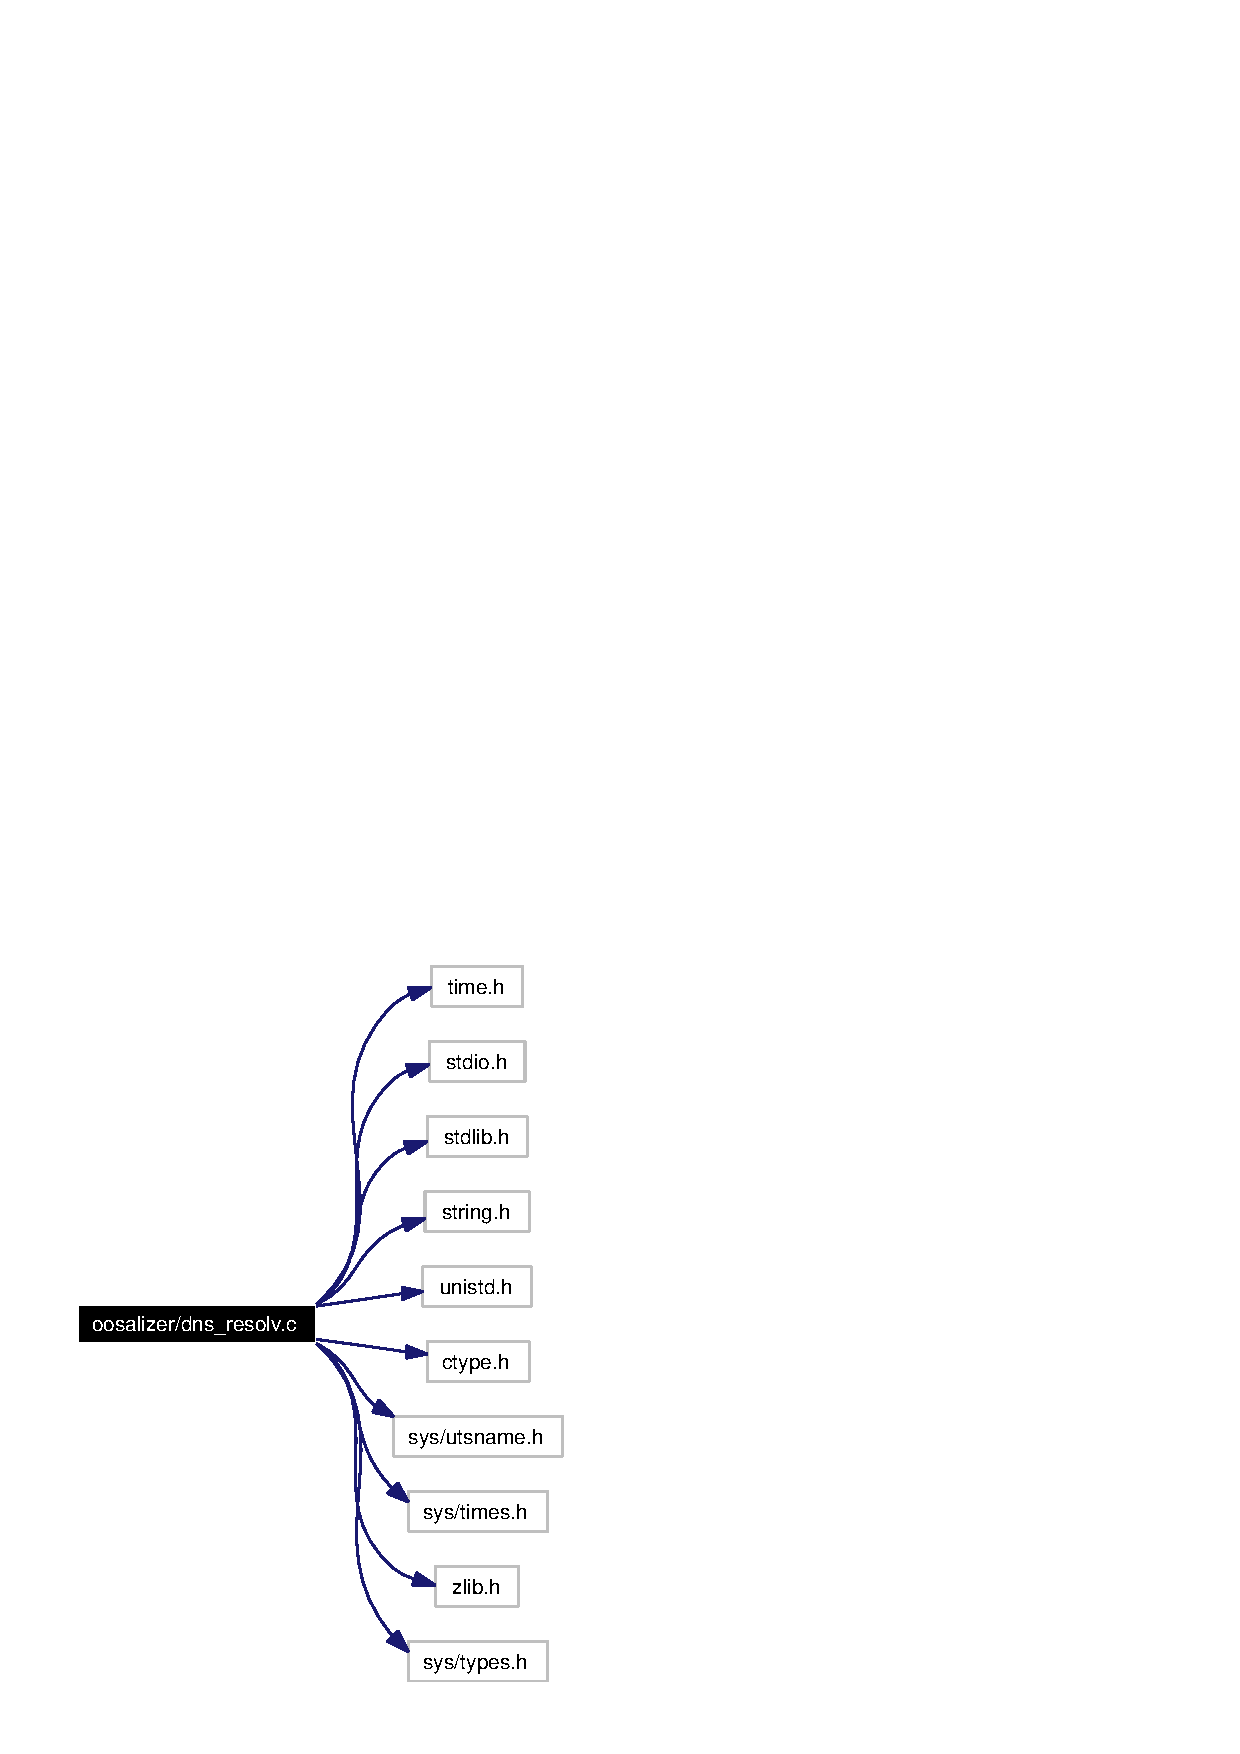
\includegraphics[width=135pt]{dns__resolv_8c__incl}
\end{center}
\end{figure}
\subsection*{Makrodefinitionen}
\begin{CompactItemize}
\item 
\#define {\bf CLK\_\-TCK}~\_\-SC\_\-CLK\_\-TCK
\end{CompactItemize}


\subsection{Makro-Dokumentation}
\index{dns_resolv.c@{dns\_\-resolv.c}!CLK_TCK@{CLK\_\-TCK}}
\index{CLK_TCK@{CLK\_\-TCK}!dns_resolv.c@{dns\_\-resolv.c}}
\subsubsection{\setlength{\rightskip}{0pt plus 5cm}\#define CLK\_\-TCK~\_\-SC\_\-CLK\_\-TCK}\label{dns__resolv_8c_03df76d1f70664d745ca8de2864e39b3}




Definiert in Zeile 71 der Datei dns\_\-resolv.c.